\mychapter{Réécriture}
\label{Cap:TD1}


\section{Description physique}
Nous avons perçu que le système demandé sur la gestion d’une voie de péage d’autoroute.
%Nous avons élaborré dans ce document une première description de système d’un péage d’autoroute.

\begin{figure}[h]
    \centering
    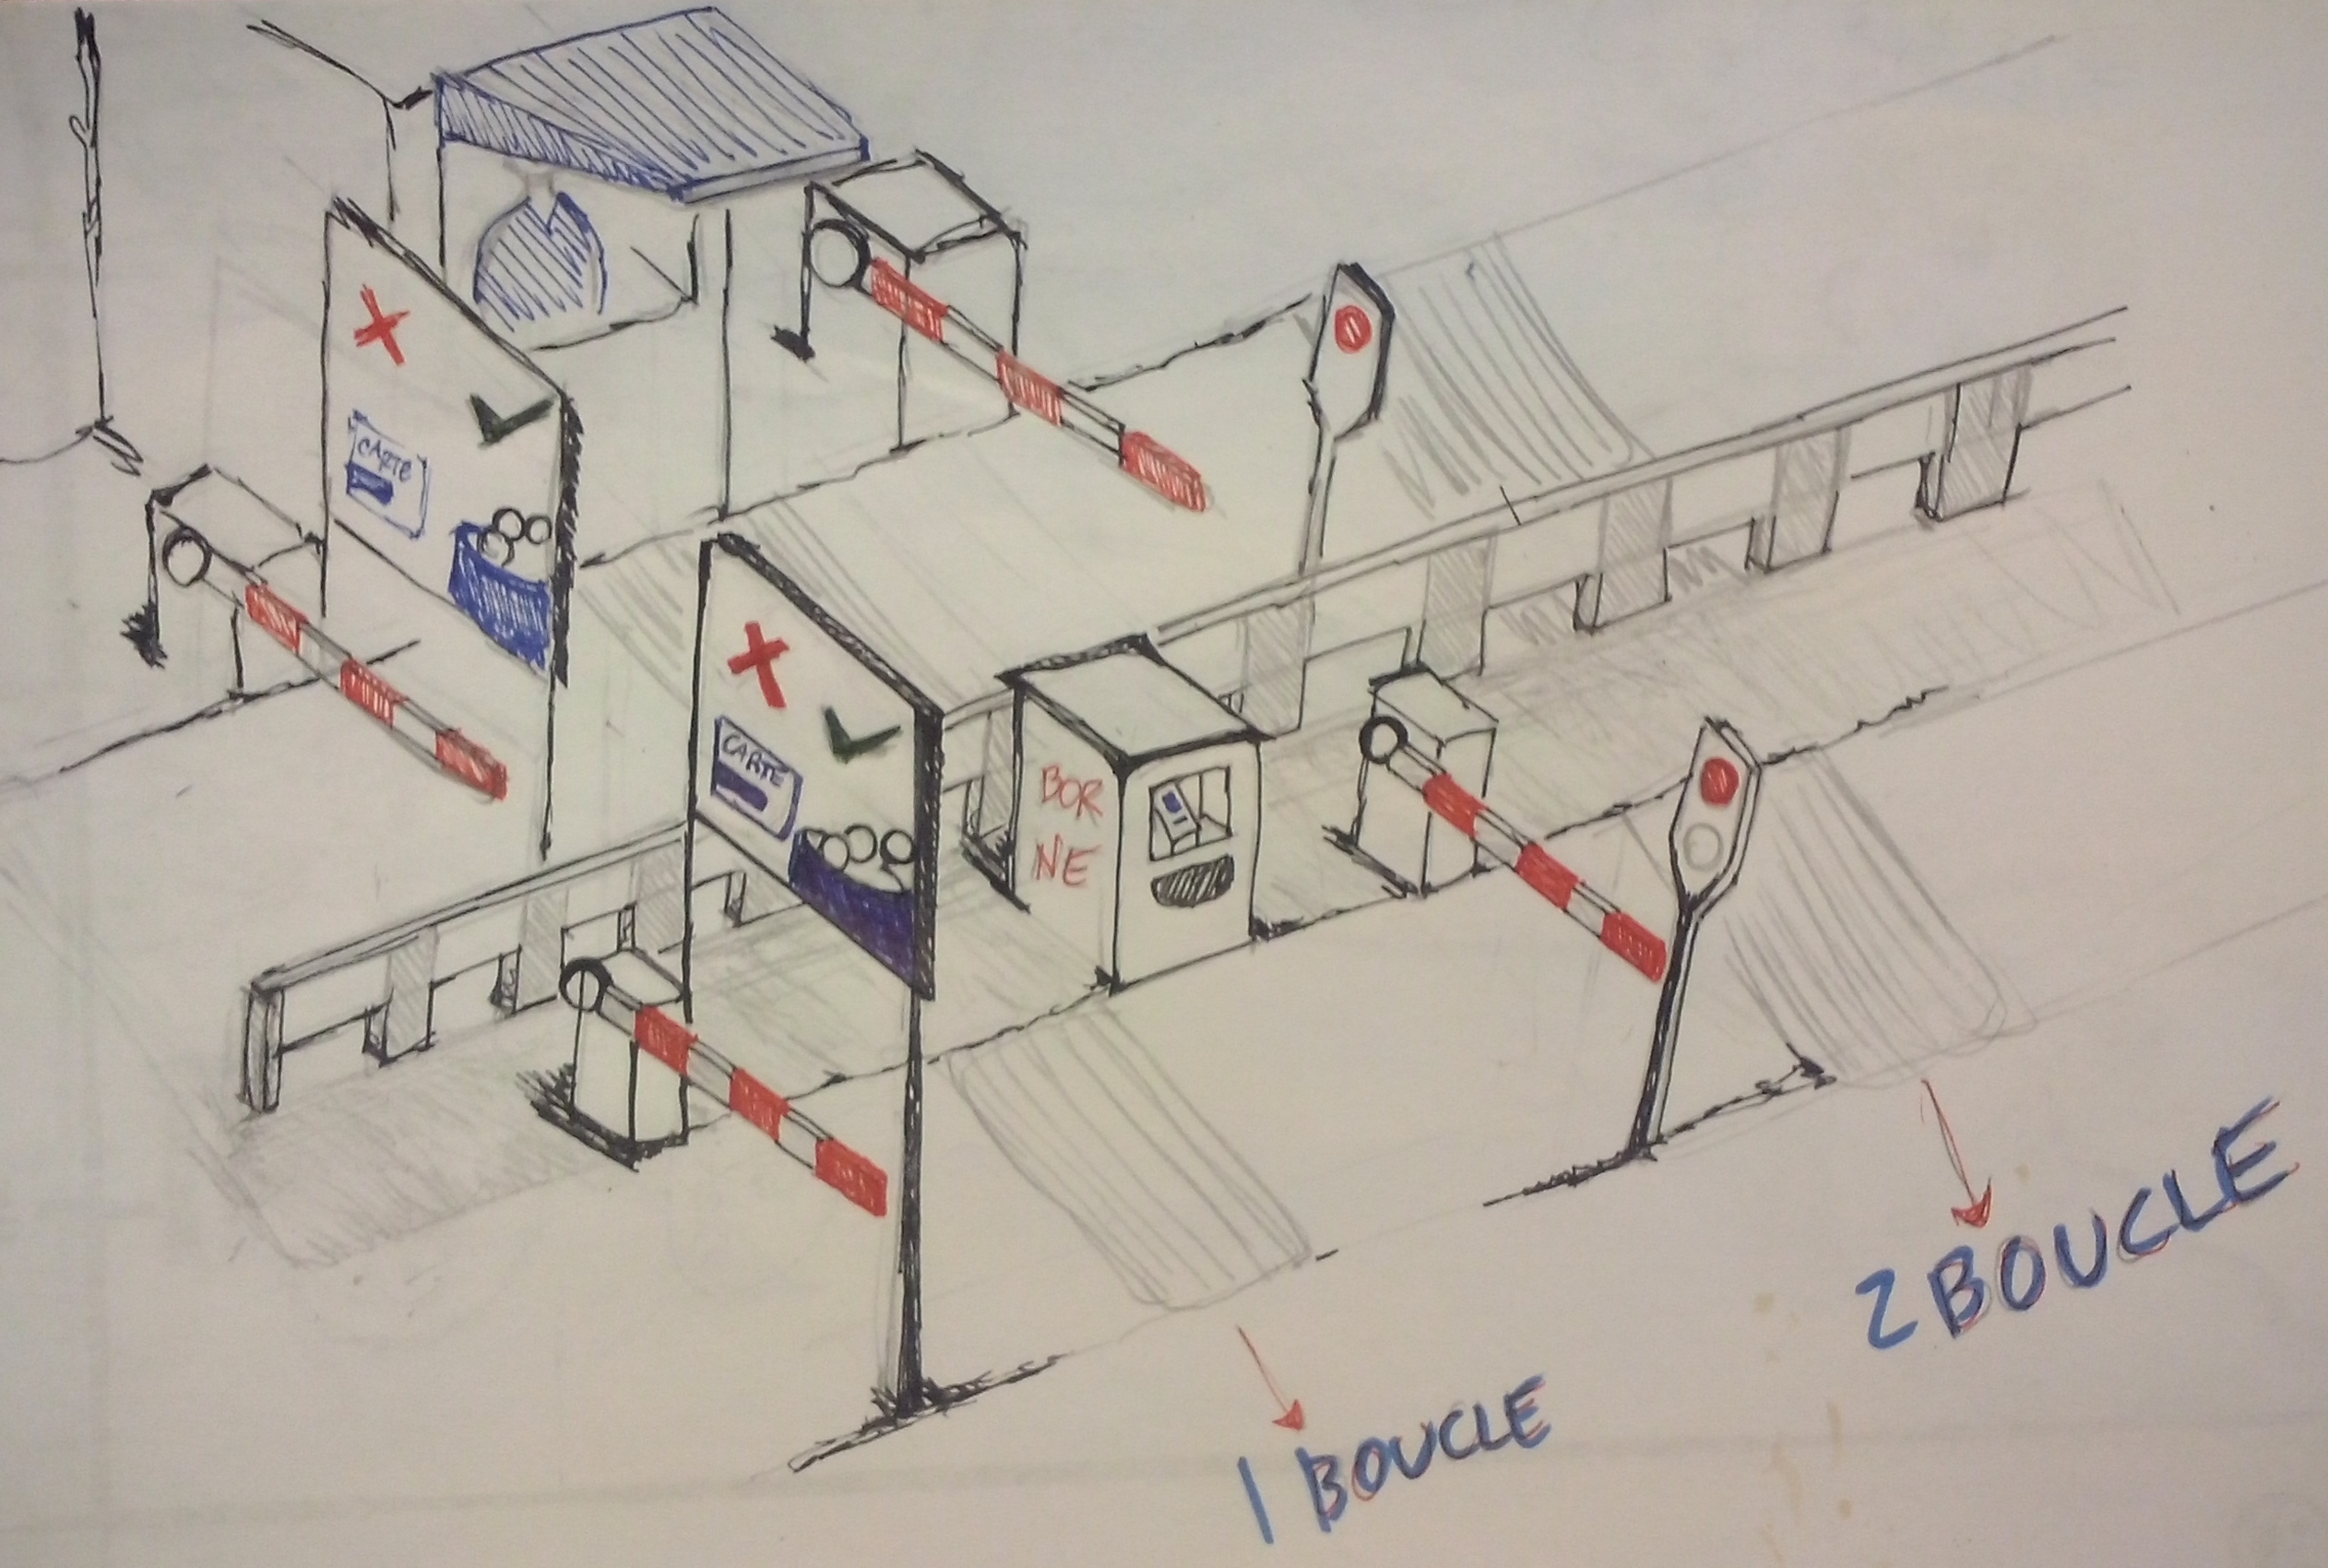
\includegraphics[scale=0.16]{02_Desenvolvimento/TD1/images/desc.png}
    \caption{Description physique}
    \label{fig:my_label}
\end{figure}
\newpage
\section{Réécriture de l'expression des besoins recentrée sur les utilisateurs du systeme}
\subsection{Les acteurs} 
Nous avons reconnu cinq acteurs (utilisateurs) du système tel que :
\begin{itemize}
    \item \textbf{Le Client (Conducteur de voiture)}: Le conducteur est le client, le rôle du conducteur est de passer la barrière de péage autoroutiere. 
    \item \textbf{La Société d’Autoroute}: 	La société est la propriétaire de la barrière de péage et gère donc la barrière. C’est elle qui va gérer aussi les cartes d’abonnement et le traitement des comptes des abonnés. 
    \item \textbf{Le Technicien}: Le technicien est l’acteur premier pour la maintenance du système. Le technicien lève la barrière manuellement en cas d’urgence. Il va faire des interventions humaines si necessaire, ex: si la barrière ne s’ouvre pas. 
    \item \textbf{Operateur humain}: L’ operateur humain reçoit le paiement du client (conducteur) dans les bornes manuelles.
    \item \textbf{Le Surveillant}: Les surveillants supervisent l’ensemble des bornes pour assurer, par exemple, qu’à tout moment il y ait une voie ouverte ou que le nombre de voies ouvertes soit proportionnel au flux de véhicules. Si le système lève une alarme vers l’ordinateur du poste de surveillance, un surveillant doit faire une intervention, comme remettre de la monnaie dans une borne et fait un compte-rendu approximatif de l’incident.
\end{itemize}
\newpage
\subsection{Les Grandes Fonctionnalités du Système}
Nous avons différencié trois grandes fonctionnalités du système:\\

\textbf{Passer le péage }(\ref{subsubsec:passerL})

\textbf{Gerer la comptapilité } (\ref{subsubsec:gerer})

\textbf{Maintenance }(\ref{subsubsec:maint})\\

Ainsi voici les scénarios informels correspondant :
\subsubsection{\textbf{Cas d’utilisation:} Passer le péage } \label{subsubsec:passerL} 
\textbf{Acteur primaire}: Le Client (le conducteur) 

\textbf{Acteur support}: La Société d’Autoroute, le technicien, l’operateur humain et le surveillant

Le client (le conducteur) opte pour une voie selon son type de véhicule et le moyen de paiement. Le client effectue le paiement selon le type de borne qu’ il a choisi (avec une carte d’abonnement, carte de crédit, monnaie, monnaie avec un opérateur humain, etc). Le système gère l’ouverture de la barrière une fois le montant payé ou la carte d’abonnement présenté, si la barrière ne s’ouvre pas, alors un technicien ou un opérateur doit venir régler l’incident survenu.


\subsubsection{\textbf{Cas d’utilisation:} Gerer la comptabilité}  \label{subsubsec:gerer}
\textbf{Acteur primaire}: La Société d'autoroute 

Le système doit assurer la comptabilité générale de l’ensemble des bornes. Chaque levée de barrière est enregistré. Les cartes d’abonnement et les compte des abonnés sont gérés par la société d’autoroute de façon instantanée, chaque passage est enregistré. Les opérations par cartes bleues sont gérées en fin de journée. Les bornes détectent les fausses pièces et les cartes volées.

\subsubsection{\textbf{Cas d’utilisation:} Maintenance}  \label{subsubsec:maint}
\textbf{Acteur primaire}: Le Technicien 

\textbf{Acteur support}: Le surveillant, l’opérateur humain

Le technicien permet de gérer toutes les cas, incidents, qui nécessitent une intervention humaine, lorsque qu’une barrière doit être ouverte ou fermée manuellement, lorsqu’un usager se retrouve coincé à la barrière de péage ou lorsqu’une borne a besoin de réglage ou de réparation (comme remettre de la monnaie).
